\documentclass[GBK]{ctexart}
\usepackage{titlesec}
\usepackage{ulem}
\usepackage{appendix}
\usepackage{mathbbold}
\usepackage{varwidth}
\usepackage{ulem}
\usepackage{caption}
\DeclareCaptionLabelSeparator{twospace}{\ ~}   %%这三条语句即可
\captionsetup{labelsep=twospace}
%\usepackage{autobreak}
%\usepackage{caption}
%\usepackage{hyperref}
\usepackage{subfigure}
\usepackage[dvipdfmx]{graphicx}
\usepackage{bmpsize}
\usepackage{CJK,CJKnumb}
%\usepackage{indentfirst}        %首行缩进宏包
%\usepackage{latexsym,bm}% 处理数学公式中和黑斜体的宏包
\usepackage{mathrsfs}
\usepackage{amsmath,amssymb}    % AMSLaTeX宏包 用来排出更加漂亮的公式
\usepackage{graphicx}
\usepackage{cases}
\usepackage{pifont}
\usepackage{txfonts}
\usepackage{cite}
\usepackage{listings}
\usepackage{xcolor}
\usepackage{url}
%\usepackage[dvipdfmx]{graphicx}
%\usepackage{bmpsize}
\pagestyle{plain}
%\newCJKfontfamily\sectioncf{\kaishu }
%\titleformat*{\section}{\LARGE\sectioncf}
\usepackage{float}
\usepackage{epstopdf}
\usepackage{fancyhdr}
%\pagestyle{fancy}
%\lhead{
%
\includegraphics[scale=0.5]{logo.png}
%}  %在此处插入logo.pdf图片 图片靠左
%%\chead{} % 页眉中间位置内容
%\rhead{
%
\includegraphics[scale=0.1]{logo1.png}
%} 页眉右边位置内容,并加粗
%\lfoot{aa}  %页脚
%\cfoot{bb}
%\rfoot{cc}
\title{东三省}
\date{}
\author{}
\pagenumbering{arabic}
\usepackage[a4paper,left=2.5cm,right=2.5cm,top=3.7cm,bottom=2.5cm]{geometry}
\usepackage{setspace}%使用间距宏包
\usepackage{booktabs}
\usepackage{colortbl}
%\usepackage{bigstruct}
\usepackage{multienum}
\bibliographystyle{unsrt}
\begin{document}
\titleformat*{\section}{\songti\zihao{4}}
\titleformat*{\subsection}{\songti\zihao{-4}}
\titleformat*{\subsubsection}{\songti\zihao{-4}}
\begin{spacing}{1.5}%%行间距变为double-space
\newcommand{\song}{\CJKfamily{song}}
%\maketitle
\zihao{-4}
%\begin{abstract}
%\zihao{-4}
%该部分内容是放置摘要信息的。该部分内容是放置摘要信息的。该部分内容是放置摘要信息的。该部分内容是放置摘要信息的。该部分内容是放置摘要信息的。

%\end{abstract}

%关键字:
%%\thispagestyle{empty}
%\setcounter{page}{3}
%\newpage
%\newcommand{\song}{\CJKfamily{song}}
\tableofcontents
\setcounter{page}{4}
%\thispagestyle{empty} % 当前页不显示页码
\newpage
\setcounter{page}{3}
\title{题目:航迹目标轨迹数据挖掘}
\maketitle
\section{问题与背景}
\subsection{背景介绍}
飞机如今已经成为了人们出行的重要交通工具\cite{zhu},不论是出差还是旅行,几乎都会把它作为首选。而及时发现空中突发的异常情况也是保护人们生命财产安全的重中之重。2018年5月14 日,四川航空公司3U8633 航班执行重庆-拉萨航班任务,在成都区域巡航阶段,驾驶舱右座前风挡玻璃破裂脱落,机组实施紧急备降。2019年7月9日上午,在由贵阳飞往北京的南航CZ3681 航班上,一位旅客突然心脏剧烈疼痛,飞机紧急备降到山西太原机场,让患者及时就医治疗。

类似的航班未依照规定航路行进的异常情况时有发生,而且随着科技的发展和航空领域的需要,为更好的智能化监控实现对飞行目标的属性识别,行为模式辨识,异常状态检测,本文将对航迹目标的活动规律、运动情况、模式判别进行研究与挖掘。

对于航迹而言,完成上述研究任务,要对空中目标的经纬度、速度、高度、速度、时间等状态进行分析和预测。目标活动规律分析是数据融合分析领域的重要课题,而实时目标模型研究和特定模式挖掘则是目标活动规律分析领域的研究重点,具体表现为对各种轨迹数据项进行理论建模并依据相似度度量方法,评估目标工作状态;解决特定模式的定量化可视化模型构建,模型间处理好相似性度量问题。

现实情况是,随着传感器和通信设备的与日俱增,人们可以实时接收发射海量数据,这为研究空中目标的运动方式与规律提供了巨大的便利。但同时由于轨迹数据量大、数据质量不一、数据收发点分布不均等特点,也给航路信息提取和航迹模式挖掘带来了困难。为此,本文将利用成熟的机器学习和数据挖掘算法,完成航迹目标活动规律挖掘研究任务。

\subsection{问题重述}
本论文将就飞行目标的实时状态评估问题和特定轨迹模式问题,进行分析、计算、设计模型、评估优化。

\subsubsection{任务一:轨迹聚类}
对Trace\_All文件包含7个目标的航迹数据处理分析,针对7个不同目标提取所有的航路信息。%
\subsubsection{任务二:轨迹分类与异常检测}
对Trace\_for\_Compute\_Similarity文件包含3个实时目标的航迹数据处理分析:
\begin{itemize}
  \item 设计目标F-X实时航迹与任务一中提取的航路信息相似度度量方法;
  \item 依据相似度度量方法评估实时目标工作状态;
  \item 判别目标是否出现异常。
\end{itemize}
\subsubsection{任务三:轨迹分类与异常检测}
对Trace\_All文件包含7个目标的航迹数据处理分析:
\begin{itemize}
  \item 设计算法挖掘特定模式,例如“8”字型轨迹、“S”形轨迹、圆形轨迹等;
  \item 解决模式之间相似性度量问题。
\end{itemize}
\section{符号含义与名词解释}
\subsection{符号含义}
\begin{table}[H]
  \centering
  \caption{符号说明}
    \begin{tabular}{|r|l|}
    \toprule[2pt]
    符号    & \multicolumn{1}{l|}{含义} \\
    \midrule[1pt]
    \rowcolor[rgb]{ .816,  .808,  .808} F    & 飞行目标编号(Target)\\

    T    & 航迹,由无数条航迹(ID)构成 \\

    \rowcolor[rgb]{ .816,  .808,  .808} P & 航迹点信息,五维向量 \\

    WD & 纬度 \\

    \rowcolor[rgb]{ .816,  .808,  .808} JD & 经度\\

     GD  & 高度 \\

    \rowcolor[rgb]{ .816,  .808,  .808}SD  & 速度 \\
     SJ& 时间 \\
    \rowcolor[rgb]{ .816,  .808,  .808}k& 聚类个数 \\
    ${\beta _k}$& 聚类结果 \\
    \rowcolor[rgb]{ .816,  .808,  .808}${\alpha _k}$& 聚类中心\\
    $\bar V$&平均速度\\
     \rowcolor[rgb]{ .816,  .808,  .808}$S{C_i}$&速度修正系数\\
    $T{C_i}$    & 修正后的轨迹 \\
    \rowcolor[rgb]{ .816,  .808,  .808}  $r(T{C_i},T{C_0})$& 相似度度量函数  \\
    ${H_{_{ij}}}$& 能量高度\\
    \rowcolor[rgb]{ .816,  .808,  .808}
    $\overline {H{C_j}}$&  能量高度中心\\
    $H{C_{ij}}$ & 修正后的能量高度 \\
   \rowcolor[rgb]{ .816,  .808,  .808}$\overline {di{s_i}}$    & 能量高度轨迹的异常点到能量高度中心轨迹对应点的平均距离\\
   % ${\left. {{f_{(1)}}} \right|_{(i,j)}}$ & 每一个观测值与期望值35dbm的距离的平方 \\
%    \rowcolor[rgb]{ .816,  .808,  .808}${\left. {{f_{(2)}}} \right|_{(i,j)}}$& 每一个观测值与附近观测值的均值距离的平方 \\
%    ${n_{close}}$       & 32个单元中关闭的单元数 \\
%    \rowcolor[rgb]{ .816,  .808,  .808}${N_{close}}$      & 32个单元中关闭的单元数函数 \\
%    F     & 微波问题2的目标函数 \\
%    \rowcolor[rgb]{ .816,  .808,  .808}${P_m}$ & 遗传算法中的变异概率 \\
%    ${R^2}$ & 可决系数 \\
%    \rowcolor[rgb]{ .816,  .808,  .808}${x_{pq}}$ & 第p个样本的第q个指标的数值 \\
%    ${Y_{pq}}$ & 熵权法指标标准化处理结果 \\
%    \rowcolor[rgb]{ .816,  .808,  .808}${P_{pq}}$ & 第q项指标下第p个样本值占该指标的比重 \\
%     ${E_q}$ & 第q项指标的熵值 \\
%    \rowcolor[rgb]{ .816,  .808,  .808}${d_q}$ & 第q项指标信息熵的冗余度(差异) \\
%    ${W_q}$ & 各项指标的权重 \\
%    \rowcolor[rgb]{ .816,  .808,  .808}${S_p}$ & 各样本的综合得分 \\
%    ${\rm{w(u, v)}}$  & 最小生成树算法中边的权重 \\
%
%    \bottomrule[2pt]
%    \end{tabular}%
%  \label{tab:addlabel}%
%\end{table}%
%\begin{table}[H]
%  \centering
%  \caption{符号说明续表}
%    \begin{tabular}{|r|l|}
%    \toprule[2pt]
%    符号    & \multicolumn{1}{l|}{含义} \\
%    \midrule[1pt]
%    \rowcolor[rgb]{ .816,  .808,  .808}c     & 弧的容量 \\
%    f     & 弧的流量 \\
%    \rowcolor[rgb]{ .816,  .808,  .808}G = (V, E) & 无向图 \\
%    V     & 点集 \\
%    \rowcolor[rgb]{ .816,  .808,  .808}E     & 边集 \\
%    $v_{s}$ & 源点 \\
%    \rowcolor[rgb]{ .816,  .808,  .808}$v_{t}$ & 汇点 \\
%   y& 不同调制格式的使用数目 \\
%   \rowcolor[rgb]{ .816,  .808,  .808}${\rm{cost(x)}}$& 价值函数\\
%   $\eta $& 折减系数 \\
    \bottomrule[2pt]
    \end{tabular}%
  \label{tab:addlabel}%
\end{table}%
\subsection{名词解释}
\begin{itemize}
  \item 航路\cite{hl}:由国家统一划定的具有一定宽度的空中通道。有较完善的通信、导航设备,宽度通常为20KM。划定航路的目的是维护空中交通秩序,提高空间利用率,保证飞行安全。
  \item ADS-B数据\cite{ads}:ADS-B全称是Automatic Dependent Surveillance - Broadcast,中文是广播式自动相关监视,顾名思义,即无需人工操作或者询问,可以自动地从相关机载设备获取参数向其他飞机或地面站广播飞机的位置、高度、速度、航向、识别号等信息,以供管制员对飞机状态进行监控。
\end{itemize}
\section{任务一:提取航路信息}
\subsection{飞行目标异常行为定义}
智能监控下的异常行为监测是一个备受关注的领域,总结各种领域对异常检测的研究可以大体把飞行目标的异常行为检测分为两大部分:

对于数据采集:由于收发设备的对信号信息传输的稳定可靠性不同、设备采集点地理位置分布不合理、网络通信的异常导致的数据收集的不可靠、不可用、不完整等异常;

对于实体飞行目标行为检测:不同于其他常见的智能监控研究领域中的异常行为检测情景,例如平面二维问题如地面车辆\cite{car}、船舶航海航线\cite{ship}问题,飞行目标的运动状态是多维度立体的问题。于是,本文将把飞行目标的异常行为检测划分为水平面和铅垂面两个平面来观察监测运动状态和轨迹位置的异常情况,具体分类见下图:
\begin{figure}[H]
  \centering
  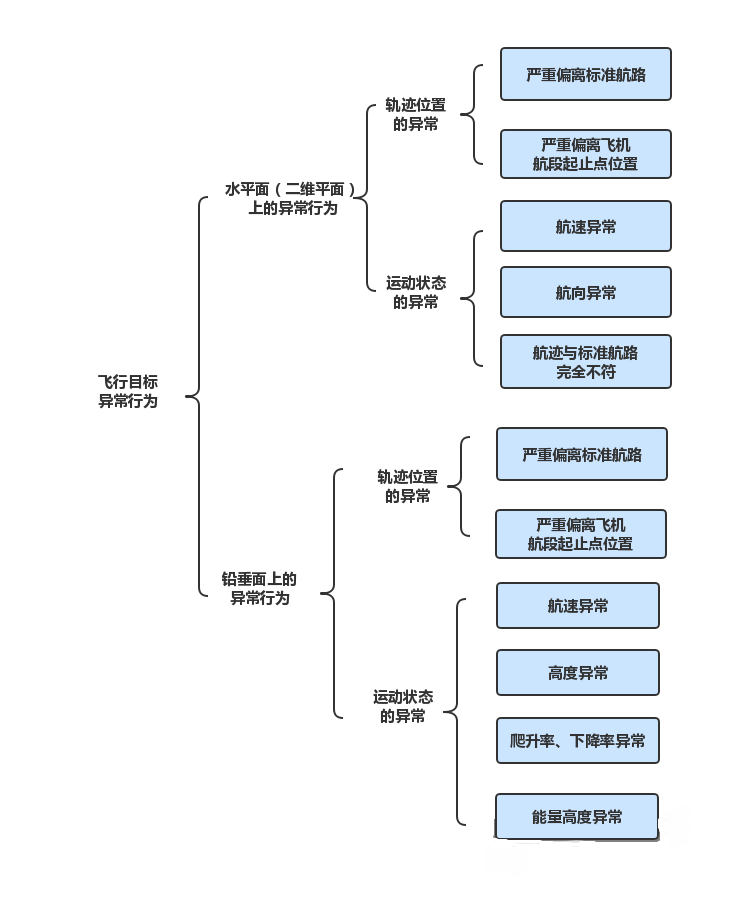
\includegraphics[scale=0.85]{yi}\\%,natheight=210
  \caption{飞行目标异常分类}\label{yi}
\end{figure}
\subsection{问题分析}
首先,为了提取所有的航路信息,先对F-1到F-7共7个历史运动轨迹进行数据处理和规律挖掘。

航空器的飞行轨迹数据一般是通过雷达、ADS—B监视设备等采集得到,理想化情况下由一组具有相同时间间隔的离散点构成。每个飞行轨迹数据除了包含时间t与空间(x,y,z)信息,有时还包括航向、速度等飞行特征信息,是一种典型的高维数据。考虑到实际航迹数据更加复杂,比如在查阅挖掘了网页\cite{map}\cite{aware}上的ADS-B数据发现真实情况中的航迹数据由于志愿者们的定位通信设备的精确度有限,ADS-B信息收发点的地理位置分布不均匀(如海上、高山等人迹罕至的地方以及无人类资源开发涉及处的位置缺乏ADS-B 信息收发点),导致航路信息的采集频率并不固定,航迹段的数据经常出现缺失现象。所以实际情况下的轨迹数据,其空间和时间信息不确定性互相影响,对采集到的数据的分析带来了困难。本题提供的仿真民航数据每10秒一条,理想化的采样频率方便更广泛的数据规律挖掘方法的研究分析。同时,所有航迹的速度数据均介于650km 和750km之间,高度数据均介于4500km和5500km之间。说明航迹是飞机完整航班也即从起飞到降落的航路中的一部分,即不包含类似起飞和降落阶段高度明显变化的部分。
\subsection{模型建立及数据处理}
飞行目标的轨迹数据作为发掘航路信息的重要时空数据,它能够反映飞行目标的历史位置、速度、高度等信息。F-1到F-7共7个飞行目标的历史运动轨迹地图散点图见下页图\ref{quantiyuanshi}。以下给出数据处理的步骤:
\begin{figure}[h]
  \centering
  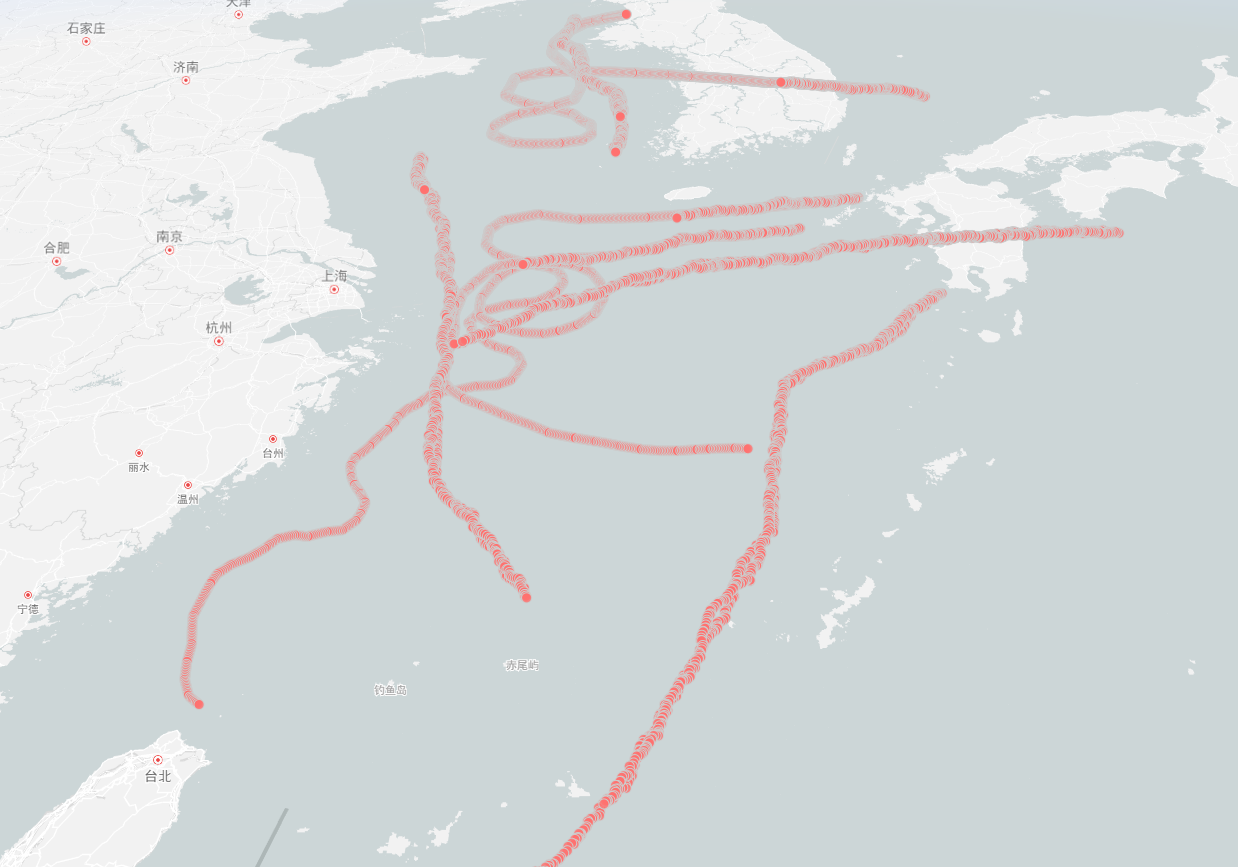
\includegraphics[width=15cm,height=8cm]{quantiyuanshi.png}\\
  \caption{七个飞行目标轨迹地图散点图}\label{quantiyuanshi}
\end{figure}
1、按照七个目标分类:针对每一个飞行目标的所有历史轨迹进行研究,存入子表格中。为了不失一般性,航迹表示为
\begin{equation}
F=\left\{T_{1}, T_{2}, \cdots, T_{i}, \cdots, T_{n}\right\}
\end{equation}
式中,$T_{i}$为第i条航迹;i∈[1,n]为航迹编号;n为航迹总条数。且$T_{i}$可用航迹点的数据集表示为
\begin{equation}
T_{i}=\left\{P_{i 1}, P_{i 2}, \cdots P_{i j}, \cdots, P_{im}\right\}
\end{equation}
式中,$P_{i j}$表示第i条航迹中第j个航迹点的信息;j∈[1,m]为航迹点编号;m为航迹点总数。每一个航迹点$P_{i j}$定义为一个5维向量,即
\begin{equation}
P_{i j}=(x, y, z, v, t)
\end{equation}
式中,x、y、z、v、t分别表示第i条航迹中第j个航迹点的纬度(WD)、经度(JD)、高度(GD)、速度(SD)、时间(SJ)。

2、将本题所给的五维数据信息:纬度(WD)、经度(JD)、高度(GD)、速度(SD)、时间(SJ),进行处理。在数据处理过程中,发现只研究二维水平面上经纬度信息时,由于F-1、F-2、F-3 的经纬度不是单值函数一一对应的关系,也即由于轨迹的形状特殊性,出现了S 形、“8”字形、圆形的轨迹,在拟合标准航路的过程中会出现同一个纬度值对应两个经度值的现象,因而转而采用参数方程的思想来处理轨迹信息。可将纬度(WD)、经度(JD)、高度(GD)、速度(SD)作为因变量,进行时间到这些变量的映射。给定时间点t,通过设定以时间t作为自变量的函数WD(t)、JD(t)、GD (t)、SD(t),可以相应的求出飞行目标在时间点t 那一刻,在三维空间中的位置以及运动动态信息。

3、轨迹时间序列的标准化处理:虽然飞行目标的数据信息均为每10秒一条,但同一目标的不同航次的点迹数不同,这将无法保证对轨迹点对的匹配的有效性和合理性,因此,按照时间序列标准化处理每个航次不同的点迹信息。把每个航次的序列数除以当次航次的总航迹点数,这样把时间标准化到$\left[ {0,1} \right]$之间,这样使得同一目标的不同航次具有可比性。

其中飞行目标F-2的经过上述步骤处理后的图如下:
\begin{figure}[H]
  \centering
  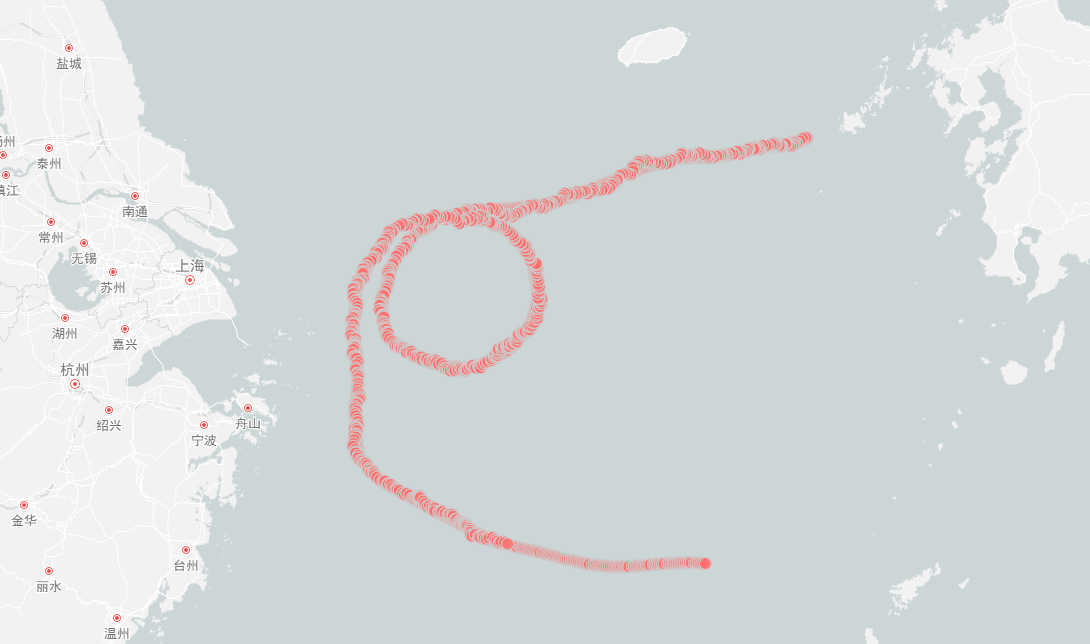
\includegraphics[width=15cm,height=8cm]{20}\\
  \caption{飞行目标F-2轨迹预处理图}\label{20}
\end{figure}
4、K-medoids航迹聚类算法:
考虑到每一条航迹数据都是由一系列的航迹点组成,航迹点数目可能都不相同,不具备典型的数据与属性之间的对应关系特征,因此,本文选用基于K-medoids划分的聚类算法,流程图如下:
\begin{figure}[H]
  \centering
  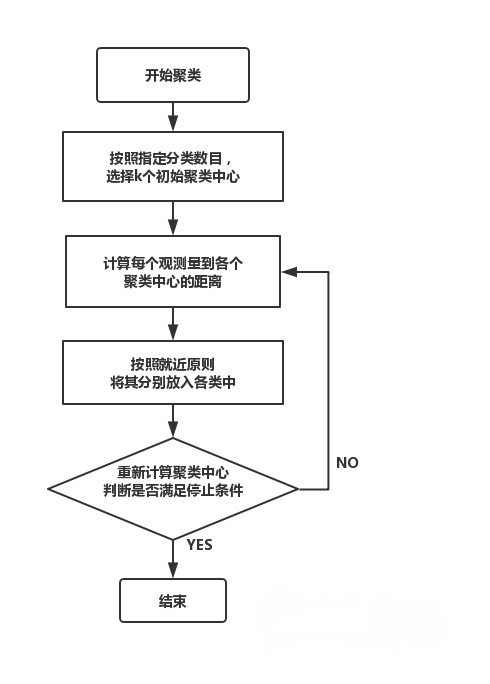
\includegraphics[width=9cm,height=9.5cm]{liuk.png}\\
  \caption{K-medoids聚类处理流程图}\label{liuk}
\end{figure}
对满足指定条件的航迹数据集进行航迹相似度的聚类分析。由于航迹的离散性,K-medoids 算法在航迹簇中选取真实的航迹作为簇中心,能很好地采用该方法结合航迹数据进行聚类。表\ref{k} 给出结合航迹数据的K-medoids算法。
\begin{table}[H]
  \centering
  \caption{K-medoids航迹聚类算法}
    \begin{tabular}{ll}
    \toprule[2.5pt]
    \textbf{输入:} & 航迹点数集合R,聚类个数k \\
    \textbf{输出:} & 聚类结果${\beta _k}$和聚类中心${\alpha _k}$ \\
    \midrule[1pt]
    步骤一:  & 随机在R中选取k个数据作为聚类中心${\alpha _k} = \{ c_1^1,c_2^2, \ldots ,c_k^1\} $  \\
    步骤二:  & 将余下的航迹根据距离簇中心点最近的原则分配到${\beta _k} = \{ C_1^1,C_2^2, \ldots ,C_k^k\} $  \\
    步骤三:  & i=2 \\
          & While($d(a_k^i,a_k^{i - 1}) > \varepsilon  \wedge i \le G$)$\{ $ \\
          & 更新簇中心$\alpha _k^i$; \\
          & i = i+1; \\
          &$\} $\\
    步骤四:  & 输出聚类结果${\beta _k} = \beta _k^G = \{ C_1^G,C_2^G, \ldots ,C_k^G\} $ 和聚类中心${\alpha _k} = \{ c_k^G,c_2^G, \ldots ,c_k^G\} $\\
    \bottomrule[2.5pt]
    \end{tabular}%
  \label{k}%
\end{table}%
其中,F-2目标聚类后轨迹见下图,用紫色点表示,可以看到聚类效果很好,已经完成了把大量多次航次的航迹点统一出标准航路的雏形。
\begin{figure}[H]
  \centering
  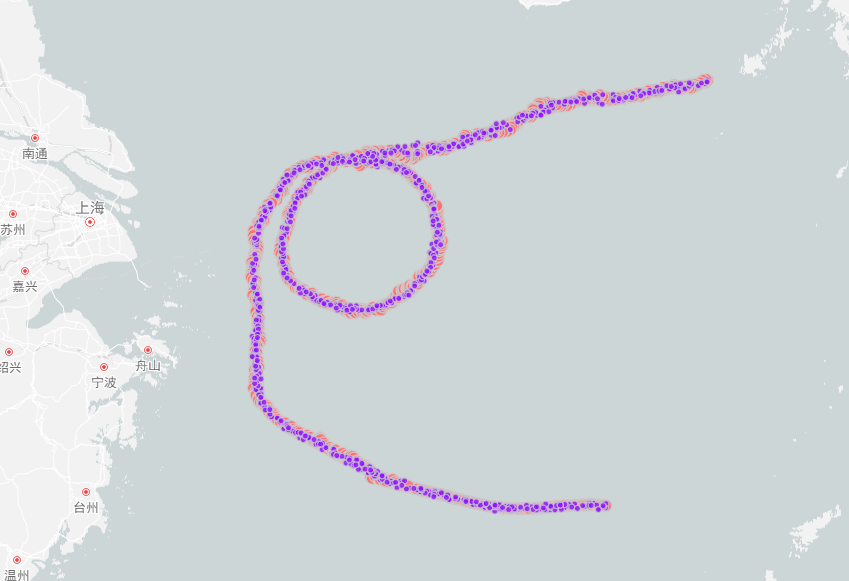
\includegraphics[width=15cm,height=8cm]{21}\\
  \caption{飞行目标F-2聚类结果图}\label{21}
\end{figure}
5、使用matlab采用傅里叶8阶标准函数形式为!!进行函数拟合,其中F-2聚类后的标准航路的拟合公式为:

拟合结果图如下:
\begin{figure}[H]
  \centering
  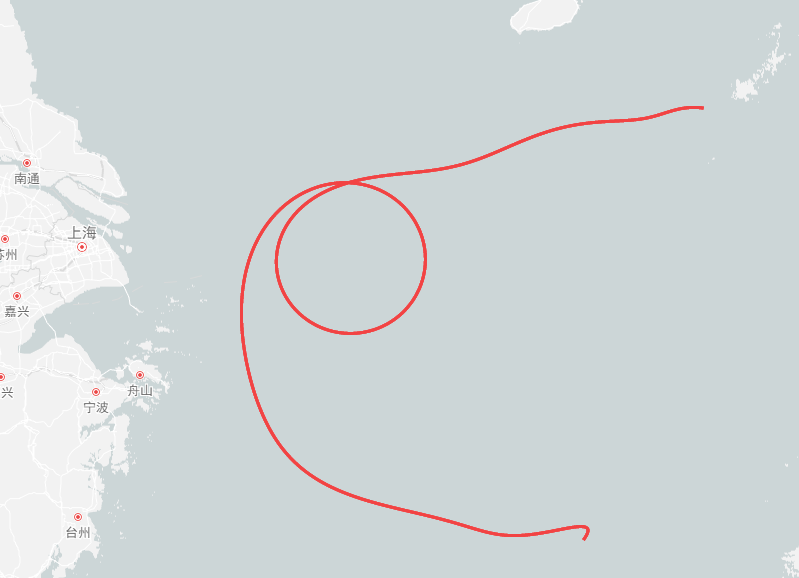
\includegraphics[width=15cm,height=8cm]{22}\\
  \caption{七个飞行目标拟合结果图}\label{22}
\end{figure}
把F-2飞行目标的原始预处理后的点迹、聚类后的点迹、拟合后的标准航路示意图现统一放于同一个地图上,
\begin{figure}[H]
  \centering
  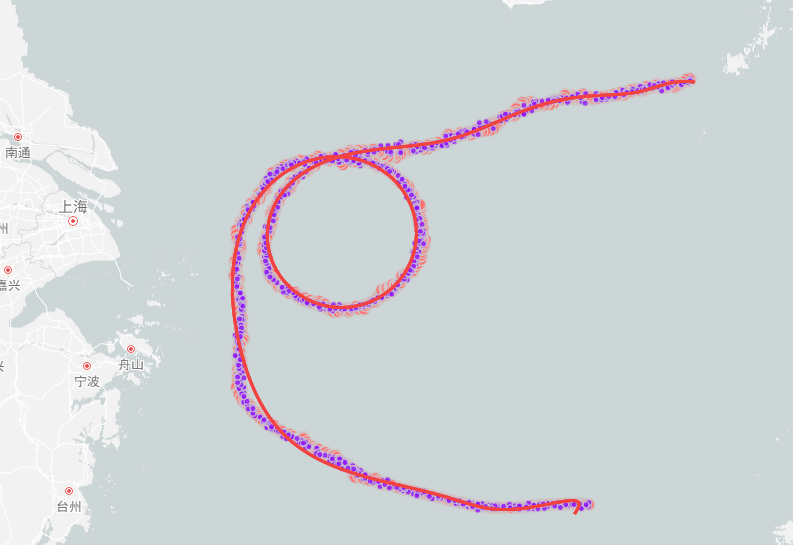
\includegraphics[width=15cm,height=8cm]{23}\\
  \caption{七个飞行目标拟合结果图}\label{23}
\end{figure}
可观察到上述处理步骤较好地完成了任务一的针对某一区域(范围在纬度(),经度())某一目标(如F-2飞行目标)的航路信息的提取工作。
对于7个目标的航迹地图可视化拟合效果如下图:
\begin{figure}[H]
  \centering
  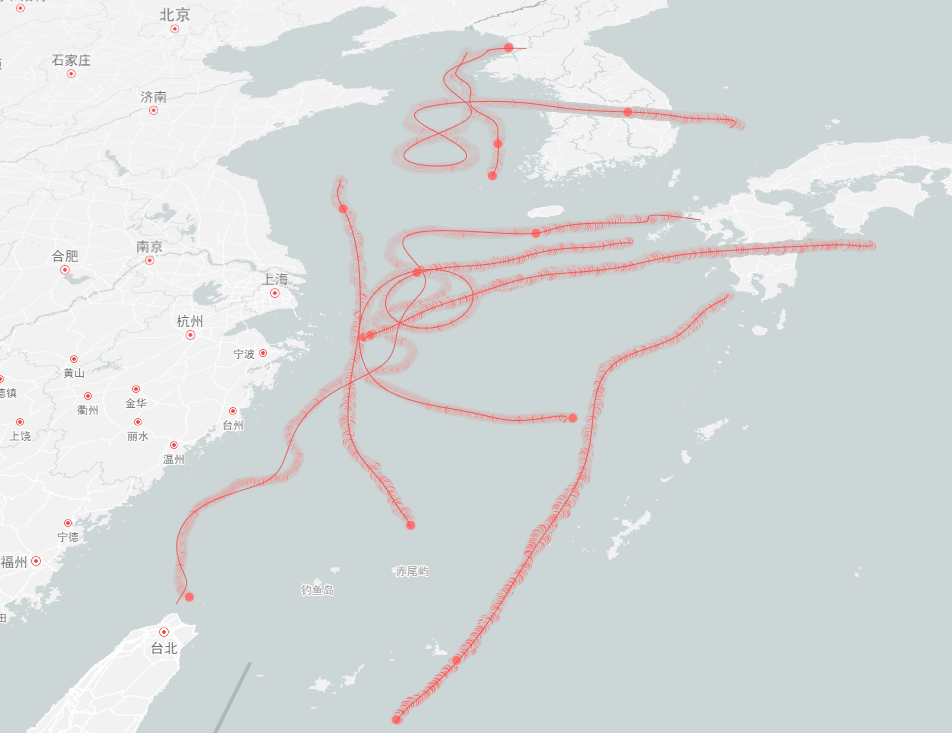
\includegraphics[width=15cm,height=8cm]{quantinihe}\\
  \caption{七个飞行目标拟合结果图}\label{quantinihe}
\end{figure}

\section{任务二:轨迹相似度度量问题}
\subsection{归一化处理}
\begin{itemize}
  %\item 先将聚合出来的点拟合成曲线。????
  \item 计算所有航迹线的飞机平均速度:
  \begin{equation}
\bar V = \frac{1}{{m \times n}}\sum\limits_{i = 1,j = 1}^{i = n,j = m} {{v_{ij}}}
\end{equation}其中,i表示第i条航迹线,j表示航迹线的第j个采样点。
  \item 计算每条航线的飞机平均速度:
   \begin{equation}
{V_i} = \frac{1}{m}\sum\limits_j^m {{v_{ij}}}
\end{equation}
  \item 设采样点数为P,计算所有航迹线的平均采样点数:
  \begin{equation}
\overline P  = \frac{1}{n}\sum\limits_{i = 1} {{P_i}}
\end{equation}
  \item 计算每条航线的运行时间:
  \begin{equation}
{t_i} = {P_i} \times \Delta t
\end{equation}其中$\Delta t$表示采样间隔(10s)。
  \item 计算速度修正系数:
  \begin{equation}
S{C_i} = \frac{{\overline V }}{{{V_i}}}
\end{equation}

  当速度较大的时候,两个采样的间隔会较大,相应的$S{C_i}$就小,通过平均速度和实际该条航迹的速度的比值将间距缩短,从而保证航迹点之间的相似度比较是在同一位置上比较。
  \item 实际航线与理论航线比较时的取点间隔即新的时间间隔为
  \begin{equation}
    t{c_i} = \frac{{{t_i}}}{{\overline P }} \times S{C_i}
\end{equation}
\end{itemize}
\subsection{基于离散的弗雷歇距离的相似度}%整理数据重新取点
按$t{c_i}$间隔重新取点记为$P{C_{{\rm{ij}}}}$,修正完的航迹线就可以表示为$T{C_i}$
\begin{equation}
    T{C_i} = \{ P{C_{i1}},P{C_{i2}},...,P{C_{ik}},...,P{C_{im}}\}
\end{equation}
使得两条航迹线处理后具有相同的维度。

查阅大量文献可知一般的轨迹相似性度量方法分为三个大类:一是相对简单的比较适合于路网静态匹配的离散点集匹配;二是通常应用于GPS序列和导航路线相似性的曲线拟合匹配,又可以细分为基于几何信息、基于拓扑信息、基于概率预测等等;三是对于时空轨迹的匹配。

由于时空轨迹相似性度量主要依赖于轨迹之间距离的定义\cite{ff},轨迹之间的距离通过轨迹之间的匹配程度来表示,不同的轨迹匹配度量方法对轨迹之间的匹配程度有着不同的处理方式。目前主流研究把时空轨迹相似性度量方法又细分为两类:基于轨迹点的相似性度量方法和基于轨迹段的相似性度量方法,如图\ref{ff}所示。
\begin{figure}[H]
  \centering
  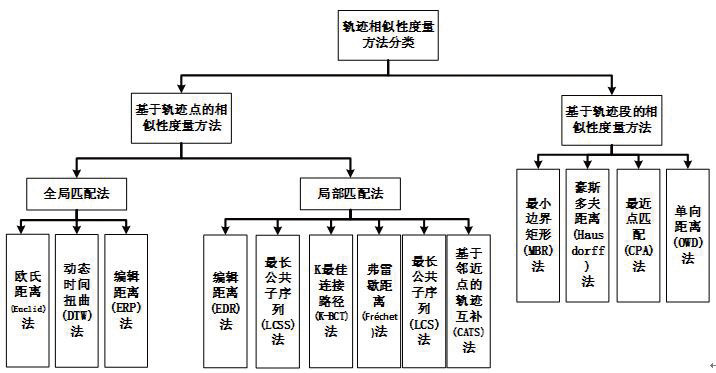
\includegraphics[scale=0.65]{ff}
  \caption{轨迹相似性度量方法分类}\label{ff}
\end{figure}

由于轨迹目前主要是以轨迹点的方式进行接收、存储,当人们对轨迹进行相似性度量时,最直观的方式就是利用两条轨迹中对应轨迹点之间的距离来度量轨迹之间的相似性。基于轨迹点的相似性度量方法种类较多,而且每种方法都有自己独特的应用场景和对相似性的定义,如有些度量方法认为两条轨迹只需要有部分相似,它们就是相似的;一些度量方法认为两条轨迹整体都相似,它们才是相似的。因而又可以基于轨迹点的相似性度量方法分成两类:全局匹配度量法和局部匹配度量法。

全局匹配法针对本文研究情景效果并不好,原因有:轨迹的采样率以及轨迹点的个数必须一致;对轨迹进行匹配时需要满足单调连续的原则;由于需要计算每一个轨迹点与其匹配点之间的距离,嗓声点也需要找到相应的匹配点,所以全局匹配方法通常对噪声都比较敏感,在实际应用中很少直接运用其计算轨迹之间的相似性。综上所述,只有当两条轨迹整体相似时才能被全局匹配度量法判定为相似。常见的全局匹配度量法比较见下图:
\begin{figure}[H]
  \centering
  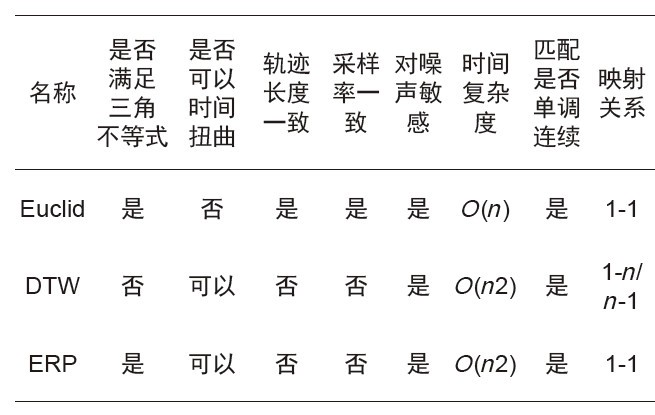
\includegraphics[scale=0.65]{quanju}
  \caption{全局匹配度量法分类}\label{quanju}
\end{figure}

由于全局匹配法在识别只有部分相似的轨迹问题上的缺陷性,本文采用局部匹配方法来研究航迹相似度度量问题。常见的局部匹配度量法的比较见下图:
\begin{figure}[H]
  \centering
  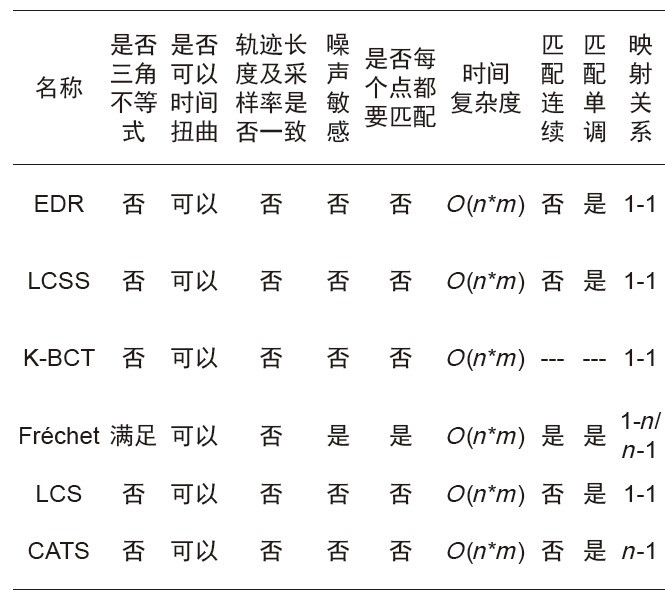
\includegraphics[scale=0.65]{jubu}
  \caption{局部匹配度量法分类}\label{jubu}
\end{figure}
本文将以基于弗雷歇距离算法\cite{flx}对航空目标多维度信息进行研究。1906年法国数学家Maurice  René   Fréchet提出了一种基于空间路径相似度描述方式,其着重将路径空间距离考虑进去,在对于有一定空间时序的曲线相似度范围的研究领域中,相较于其他局部匹配度量法的评价效率更高,这便是Fréchet distance (弗雷歇距离)。

弗雷歇距离可以直观理解为人遛狗时的狗绳距离。如图\ref{flx}所示:人在一条曲线上行走,而狗在另一条曲线上行走。前进时狗和人速度和方向可以任意改变,甚至停止,但不能倒退。弗雷歇距离指的是能够遍历两条曲线所需的最小绳子的长度。弗雷歇距离方法对采样率和轨迹长度没有要求。
\begin{figure}[H]
  \centering
  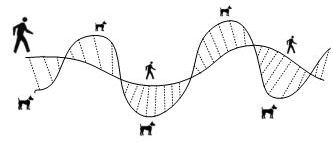
\includegraphics[scale=0.8]{flx}
  \caption{人遛狗时的绳子距离变化示意图}\label{flx}
\end{figure}
\subsection{定义轨迹相似度度量方法}
1、前面处理好的实际航线$T{C_i}$内有一个新划分的采样点$P{C_{ij}}$,现在计算它到理论航线$T{C_0}$ 内的三个点$P{C_{0j{\rm{ - }}1}}$,$P{C_{0j}}$,$P{C_{0j{\rm{ + }}1}}$的距离$d(P{C_{ij}},P{C_{0(j - 1)}})$,$d(P{C_{ij}},P{C_{0j}})$,$d(P{C_{ij}},P{C_{0(j{\rm{ + }}1}})$。其中这三个点是与实际航线的相同序列数对应下的理论航线的相应点$P{C_{0j}}$及相邻两点$P{C_{0j{\rm{ - }}1}}$,$P{C_{0j{\rm{ + }}1}}$。

2、定义相似度距离函数
\begin{equation}\label{e0}
   r(T{C_i},T{C_0}) = \frac{1}{m}\sum\limits_{j = 2}^{m - 1} {(\frac{{d(P{C_{ij}},P{C_{0(j - 1)}}) + d(P{C_{ij}},P{C_{0j}}) + d(P{C_{ij}},P{C_{0(j + 1)}})}}{3})}
\end{equation}

用实际航迹线的采样点到理论航迹对应相邻三个点的平均距离来衡量俩条线的相似度,如果r越大则相似度越低。
\begin{table}[H]
  \centering
  \caption{F-2,F-3,F-4的相似度距离函数部分计算值列表}
    \begin{tabular}{lll}
    \toprule[2.5pt]
    \multicolumn{1}{l}{F-2} & \multicolumn{1}{l}{F-3} & \multicolumn{1}{l}{F-4} \\
    \midrule[1.5pt]
    194.287 & 338.1951 & 386.5414 \\
    162.5304 & 244.1177 & 277.4326 \\
    271.9177 & 227.3047 & 103.1393 \\
    548.537 & 330.0071 & 298.3892 \\
    290.6648 & 504.251 & 166.8155 \\
    100.4237 & 181.0907 & 157.8184 \\
    364.2316 & 409.3811 & 140.5293 \\
    \multicolumn{1}{l}{...} & \multicolumn{1}{l}{...} & \multicolumn{1}{l}{...} \\
    \multicolumn{1}{l}{...} & \multicolumn{1}{l}{...} & \multicolumn{1}{l}{...} \\
    \multicolumn{1}{l}{...} & \multicolumn{1}{l}{...} & \multicolumn{1}{l}{...} \\
    \multicolumn{1}{l}{...} & \multicolumn{1}{l}{...} & \multicolumn{1}{l}{...} \\
    231.1939 & 138.6843 & 210.6878 \\
    363.6303 & 193.8611 & 235.1108 \\
    463.4054 & 136.6217 & 311.7938 \\
    179.568 & 167.4875 & 309.5157 \\
    309.1877 & 272.7435 & 124.4183 \\
    124.9426 & 164.559 & 268.3349 \\
    578.1921 & 115.2399 & 213.2892 \\
    107.2284 & 514.9955 & 149.5584 \\
    279.4314 & 127.359 & 103.6578 \\
    \bottomrule[2.5pt]
    \end{tabular}%
  \label{tab:addlabel}%
\end{table}%
3、设置评判是否异常的阈值边界:由公式(\ref{e0})含义可知,其值最小值为0,因而下边界就是零。对于上边界,由国家统一划定的航路宽度为20KM,可以将上文得到的理论航线向两侧分别沿线的法向平移正负10KM形成两条新的边界航线,之后重新计算理论航线到其中一条边界航线的r 值,并把这个值当成上边界。也即公式表述为当满足下述条件时:
\begin{equation}\label{e0}
   \frac{{d(P{C_{ij}},P{C_{0(j - 1)}}) + d(P{C_{ij}},P{C_{0j}}) + d(P{C_{ij}},P{C_{0(j + 1)}})}}{3}{\rm{ = }}d(P{C_{ij}},P{C_{0j}}){\rm{ = }}10{\rm{KM}}
\end{equation}
可以得到评价飞行目标实时状态是否出现异常的上边界r值。
\subsection{铅垂面的异常识别}
1、参考文献\cite{deng}\cite{gui}为了更好的描述飞行器的高度状态,引入能量高度H概念,由机械能转换定律
\begin{equation}\label{e0}
   mgH = mgh + \frac{1}{2}m{v^2}
\end{equation}
可得:
\begin{equation}\label{e0}
   H = h + \frac{1}{{2g}}{v^2}
\end{equation}
其中g表示重力加速度取$9.8m/{s^2}$,v表示飞行目标的飞行速度。通过这样计算可以得到每一个采样点的能量高度${H_{_{ij}}}$,同上文设定的一样,i表示第i条航迹线,j表示航线上的第j个航迹点或称采样点。

2、将上述得到的能量高度轨迹重新插值得到连续的能量高度轨迹:

线性差值是一种针对一维数据的插值方法,它根据一维数据序列中需要插值的点的左右邻近两个数据点来进行数值的估计。该方法简单易行,已知两个坐标点(${t_1}$ ,h)和(${t_2}$ ,h),确定[${t_1}$,${t_2}$]时间内t的值,根据两点式直线方程,求解出航空目标的能量高度坐标
\begin{equation}
\frac{h-h_{1}}{h_{2}-h_{1}}=\frac{t-t_{1}}{t_{2}-t_{1}}
\end{equation}

其算法步骤如下:

\textbf{Step 1:}将所需要进行线性差值的表格用xlsread()语句导入MATLAB;

\textbf{Step 2:}在MATLAB 中读取进行线性差值的列;

\textbf{Step 3:}用interp1()语句进行线性差值;

\textbf{Step 4:}将用线性差值得到的航迹数据导入Excel 表中。

3、由上一步中得到的新的时间间隔${t_{ci}}$重新取点$H{C_{ij}}$,组成新的能量轨迹采样点集$G{D_i}$,$G{D_i} = \{ H{C_{i1}},H{C_{i2}},...,H{C_{ij}},...,H{C_{im}}\} $

4、计算能量高度中心:有n条航迹,每条航迹的能量高度$H{C_{ij}}$在对应的j个位置处进行加和去均值,即:
\begin{equation}
\overline {H{C_j}}  = \frac{1}{m}\sum\limits_{i = 1}^n {H{C_{ij}}}
\end{equation}
从而得到能量高度中心轨迹$G{D_0} = \{ \overline {H{C_1}} ,\overline {H{C_2}} ,...,\overline {H{C_j}} ,...,\overline {H{C_m}} \} $

5、采用盒须图的方法计算能量高度的上边界和下边界:!!是让插盒须图么????

将每条航迹j位置的能量高度$H{C_j}$进行处理,计算标准差:
\begin{equation}
\sigma _{HC}^j = \sqrt {{{\frac{{\sum\limits_{i = 1}^n {(H{C_{ij}} - \overline {H{C_j}} )} }}{n}}^2}}
\end{equation}
其中F-2飞行目标的标准差图如下,横坐标为j,即所有航迹点,纵坐标为能量高度$H{C_j}$。
\begin{figure}[H]
  \centering
  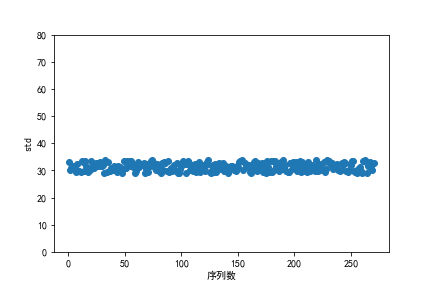
\includegraphics[width=15cm,height=8cm]{biaozhuncha}
  \caption{F-2飞行目标的标准差$\sigma _{HC}^j$图}\label{biaozhuncha}
\end{figure}
上边界计算公式为:
\begin{equation}
H{C_j}^ +  = \overline {H{C_j}}  + k \times \sigma _{HC}^j
\end{equation}

其中k表示采用几倍标准差,本文取k=2,即采用2$\sigma $原则。之后可以得到上边界的轨迹$GD_0^ +  = \{ HC_1^ + ,HC_2^ + ,...,HC_j^ + ,...,HC_m^ + \} $,之后使用相同的上文处理轨迹点的插值方法将轨迹点插值成上曲线。

同理可得下边界计算公式为:
\begin{equation}
H{C_j}^{\rm{ - }} = \overline {H{C_j}} {\rm{ - }}k \times \sigma _{HC}^j
\end{equation}
并可以得到下边界轨迹点$GD_0^{\rm{ - }} = \{ HC_1^{\rm{ - }},HC_2^{\rm{ - }},...,HC_j^{\rm{ - }},...,HC_m^{\rm{ - }}\} $,之后处理轨迹点,插值得到下曲线。

6、能量高度阈值计算:
考虑到实际情况下,每一条航迹线与中心线或多或少会有几个点“异常”,偶尔的几个点“异常”并不能说明该轨迹异常,因此要设置阈值,也即某一航迹线的异常点数超过的一定的数量才能判定为该目标飞行状态出现异常。
给出能量高度阈值计算公式:
\begin{equation}
H{C_t} = H{C_\mu } + k \times H{C_\sigma }
\end{equation}

式中,$H{C_{_t}}$表示这簇航迹的能量高度阈值,$H{C_\mu }$表示这簇航迹的能量高度均值
\begin{equation}
H{C_\mu }{\rm{ = }}\frac{1}{{n \times m}}\sum\limits_{i = 1,j = 1}^{i = n,j = m} {H{C_{ij}}}
\end{equation}

仍有k=2,$H{C_\sigma }$表示这簇航迹能量高度的标准差$H{C_\sigma }{\rm{ = }}\sqrt {{{\frac{{\sum\limits_{i = 1,j = 1}^{{\rm{i}} = n,j = m} {(H{C_{_{ij}}} - H{C_\mu })} }}{{n \times m}}}^2}} $。
\begin{figure}[H]
  \centering
  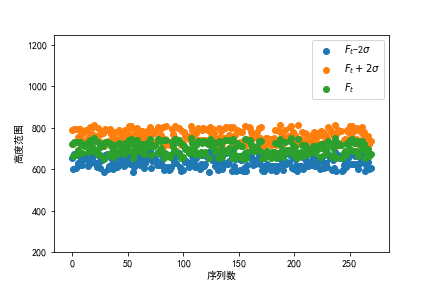
\includegraphics[width=15cm,height=8cm]{fanwei}
  \caption{F-2高度范围图}\label{fanwei}
\end{figure}
7、计算各能量高度轨迹的异常点到能量高度中心轨迹对应点的平均距离:
\begin{equation}
\overline {di{s_i}}  = \frac{1}{b}\sum\limits_{j = 1}^b {d(H{C_{ij}},\overline {H{C_j}} )}
\end{equation}

其中b表示异常点的数目,即能量高度轨迹中的点满足$H{C_{ij}} > HC_j^ +  $或$H{C_{ij}} < HC_j^ - $,则b = b + 1,如果$\overline {di{s_i}}  > H{C_t}$,则判定该轨迹为异常轨迹。

\section{任务三:轨迹模型分类}
可以观察到本题F-2,F-3,F-4数据包含了任务要求需要识别的“8”字形、“S”形、圆形模式,而其完整段轨迹也是由各种形状模式的轨迹分段构成的。下面首先对模型给出规定与假设:
\subsection{线型轨迹}
线性的单值函数类型的轨迹应满足:
\begin{equation}
\left\{ \begin{array}{l}
X = \alpha t + C\\
Y = \beta t + C
\end{array} \right.
\end{equation}

%约束条件函数h:
%\begin{equation}\label{b4}
%  h = \left\{ \begin{array}{l}
%E(10,10) \le 0\\
%{[E(10,10) - 0]^2}
%\end{array} \right.
%\end{equation}
其中$\alpha $,$\beta $是系数,C是一个常数;
\subsection{“8”字形轨迹}
由大学物理学到的知识,“8”字形轨迹标准形式应该满足:
\begin{equation}
\left\{ \begin{array}{l}
X = r\sqrt {\cos 2\theta } \cos \theta \\
Y = r\sqrt {\cos 2\theta } \sin 2\theta \\
r = r(t)\\
\theta  = \theta (t)
\end{array} \right.
\end{equation}
其中,充分考虑到轨迹形状的对称性,如果该轨迹沿某一对称轴“上下”对称,则应有$r = a + b\sin (\frac{\theta }{2})$,其中$\theta $的换算由时间t来决定。%???

下面针对一个理想化的“8”字型轨迹示意图来分析该模式在一些物理量上具有的特点:
\begin{figure}[H]
  \centering
  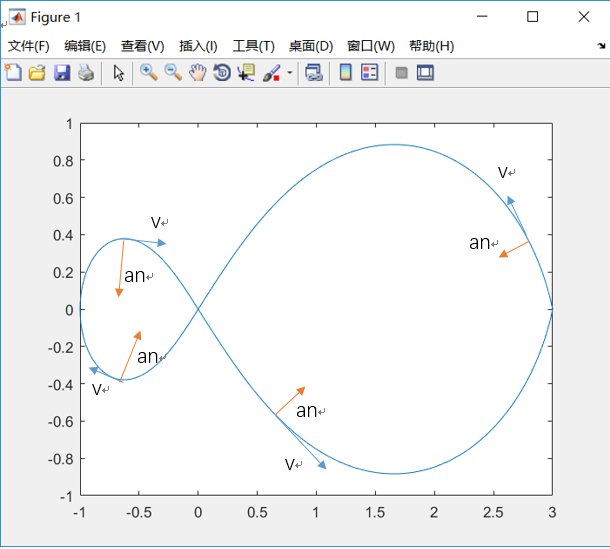
\includegraphics[width=15cm,height=8cm]{8}
  \caption{“8”字形轨迹示意图}\label{8}
\end{figure}
从图可以看到任意时刻法向加速度${a_n}$的变化情况,法向加速度${a_n}$的朝向会在交汇的点处发生变化,且在一个“周期”内会有有两次变化。现规定法向加速${a_n}$的模值函数为${A_{\rm{n}}}(t)$,观察到“8”字型轨迹模式下的${A_{\rm{n}}}(t)$会在同一位置有两个拐点。

为了不失一般性,考虑到实际情况下对于该情景的研究应注意,要排除掉同样也符合这个特点的圆形轨迹模式,二者之间的区别为“圆形”模式出现法向加速${a_n}$的模值函数${A_{\rm{n}}}(t)$ 出现两个拐点的轨迹点的距离可能过大,从而实现区别由两个“圆形”模式构成的轨迹和单独的“8”字形轨迹示意图如下:
\begin{figure}[H]
  \centering
  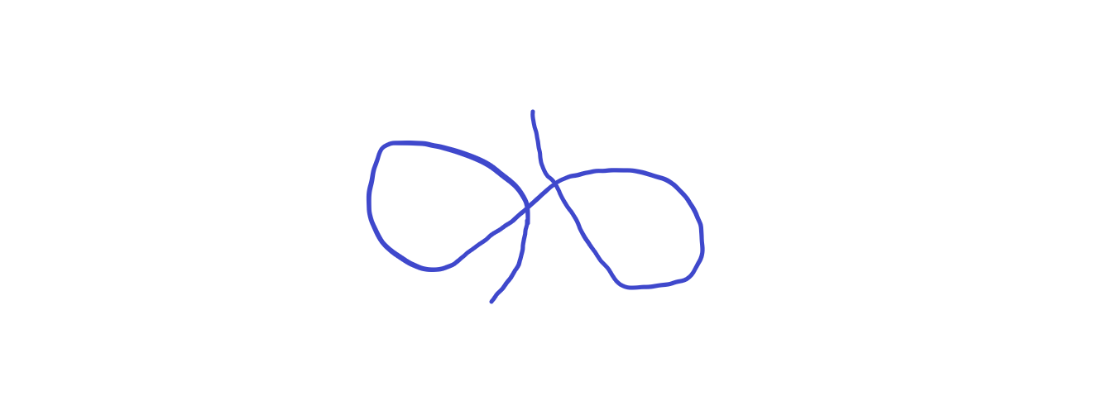
\includegraphics[width=15cm,height=7cm]{2yuan}
  \caption{类似“8”字形的“圆形”轨迹示意图}\label{2yuan}
\end{figure}

下面给出具体的公式和证明解释:由牛顿运动规律可知$\overrightarrow {{a_a}}  = \overrightarrow {{a_X}}  + \overrightarrow {{a_Y}} $运动物体的加速度可以由X方向和Y方向的加速度合成,同样也可以由切向加速度${a_\tau }$和法向加速度${a_n}$合成,本文考虑到“8”字型轨迹模式下的法向加速度${a_n}$具有可以研究识别区分与其他模式的特点,采用切向法向加速度分解法:$\overrightarrow {{a_a}}  = \overrightarrow {{a_\tau }}  + \overrightarrow {{a_n}} $。又知:${a_x} = \frac{{{d^2}x}}{{d{t^2}}}$,${a_y} = \frac{{{d^2}y}}{{d{t^2}}}$,可以求得:
\begin{equation}
{a_a}^2 = {a^2}_x + a_y^2
\end{equation}
同理可得
\begin{equation}
{a_a}^2 = {a^2}_\tau  + a_n^2
\end{equation}
其中,${a_\tau } = \frac{{dv}}{{dt}}$

%\section{模型的评价}
%\begin{itemize}
%  \item 缺点
%
%   1.微波问题1考虑了两个观测点的要求,没有过多处理辐射区域的的均匀性,以及较少关注单元的关闭通道数,无法更完美的满足工程实际中关闭尽可能多的通道降低配置成本的要求。
%
%   2.骨干网问题1,在利用熵权法处理各项指标时,由于收集到的相关可用指标较少,使得各个城市的综合评分与实际评分有一定的差距,从而使得模型预测值有一定误差。
%
%   3.骨干网问题1中的人口增长模型是通过数据拟合而成,缺乏更客观全面的分析,比如生育政策的改变,经济发展水平的影响,受教育人口分布等未来未知因素的影响,从而使得计算的信息总量有一定误差。
%
%    4.骨干网问题1中人均信息量增长模型是通过数据拟合而成,没有将新技术爆炸,经济发展水平,受教育程度等影响引入,从而使得预测的信息总量有误差。
%  \item 优点
%
%  1.灵活且合适地使用多种算法:遗传算法、最小生成树Kruskal算法、基于深度优先搜索优化后的最大流算法。
%
%\quad \quad  其中,遗传算法通过动态随机生成初始化种群并反复迭代,结合适应度函数,两个天线单元中是否有关闭的算例表明该算法取得了很好的效果。
%
%\quad \quad   最小生成树Kruskal 算法通过寻找图的最小生成树初步优化网络,为后续的细致优化提供一个可行的初始解的大体城市连接,而且它不依赖于网络的初始结构,具有更好的适用性。
%
%\quad \quad   基于深度优先搜索优化后的最大流算法,巧妙地使用了DFS搜索,排除所有不符合条件的顶点 对,使可以调整流量的简单路径数目达到最少,从而大大优化算法的执行效率。
%
%
%  2.结合大学专业课上的分析波的合成问题的方法:针对微波问题,我们从32个单元功率和相位合成入手,利用复数可以简化矢量叠加运算的特点和《微波原理》、《电磁场和电磁波》、《天线原理》课本上的知识将该问题大大简化;在求解微波问题1 的时候使用了结构优化设计的方法,迅速简化了问题,避免了从${5^{32}}$ 天文数字的32 个天线单元不同配置的排列组合中分析,大大提高了效率,缩短了求解时间,而且还很好地运用专业课所学,将书本理论很好地与实际问题结合起来。
%
%  3.搜索收集并合理处理分析了大量国家各部门官网上的与信息、通信、网络、人口等等有利于骨干网问题求解的数据。在骨干网问题1中,使用对实际数值拟合度很高的熵权法设置不同指标的权重值,避免了其他分析指标权重值方法往往主观性过强,客观性不够的缺点,使结果可信度较高。数据来源真实,处理过程客观合理,有良好的借鉴意义。
%\end{itemize}


\nocite{*}





%\end{appendices}
\end{spacing}
\normalem
%\bibliography{re1}
\begin{thebibliography}{99}%宽度9
\bibitem{zhu} 朱雅峰.我国民航空中交通管理面临的挑战和机遇[J].科技资讯,2012(16):228-
230.
\bibitem{hl} https://baike.baidu.com/item/航路/1120077?fr=aladdin
\bibitem{ads}https://baike.baidu.com/item/ADS-B
\bibitem{car}宋耀. 交通监控视频中的车辆异常行为检测[D].南京邮电大学,2015.
\bibitem{ship}张树波, 唐强荣. 基于 AIS 数据的船舶异常行为检测方法[J].人工智能与机器人研
究, 2015,4(4),23-31.
\bibitem{map}http://map.variflight.com/origin
\bibitem{aware}https://zh.flightaware.com/
 \bibitem{flx} Fréchet M M. Sur quelques points du calcul fonctionnel[J]. Rendiconti Del Circolo Matematico Di Palermo, 1906, 22(1):1-72.
 \bibitem{hu} 胡宏宇,王庆年,曲昭伟, 等.运动目标空间模式辨识与异常交通行为检测[J]. 吉林大学学报:工学版,2011,41(6):1598-1602.
 \bibitem{ff}周星星,吉根林,张书亮.时空轨迹相似性度量方法综述[J].地理信息世界,2018,25(4):11-18. DOI:10.3969/j.issn.1672-1586.2018.04.003.
\bibitem{liu}刘朋. 基于监视数据的机动区航空器异常行为检测[D].中国民航大学,2018.
\bibitem{deng}邓人博. 基于监视数据的终端区航空器异常行为识别研究[D].中国民航大学,2018.
\bibitem{1}
\bibitem{gui}桂远洋. 低空风切变下飞机自动着陆安全控制策略研究[D].南京航空航天大学,2013.
\end{thebibliography}




\end{document}
